\addsection{Units}{\images/leadership.png}
\hypertarget{Units}{In} addition to their hero and its deck, players have a deck of unit cards which represent the armies moving with their heroes.
Every faction has access to 7 different units, each with unique stats and abilities.
Units are necessary for winning combats and fulfilling scenario goals.
Each scenario's set up instructions indicate which unit cards should be included in your initial unit deck.
Your current unit deck should be kept near the town and hero boards, clearly separated from the rest of your faction’s units.\par
Each faction unit is double-sided, with a weaker “Few” side, and a stronger “Pack” side.
“Few” units may be upgraded to “Packs” by \textbf{reinforcing} them, while taking damage in combat can subsequently reduce a unit back to its “Few” side.
Units should always be kept on their correct side when moved around or inspected.\par
A player’s unit deck may have any number of units, but only up to 5 units can be selected to fight during \hyperlink{Combatsetup}{combat set up}.
If a unit is defeated in combat, discard it from your unit deck.
After combat, return any surviving units to your unit deck.
Defeated faction units can be recruited again after being defeated.
Units may be recruited and reinforced by flipping the population token and paying the unit's recruitment \includesvg[height=10px]{\svgs/pay.svg} or reinforcement \includesvg[height=10px]{\svgs/reinforce.svg} cost.
When you do so, you can instantly recruit and reinforce \textbf{any number} of times, provided you have enough resources and the prerequisite buildings to do so.\par
\textbf{Recruiting} a unit requires that your town has a dwelling of that unit’s level or higher.
\textbf{Reinforcing} requires that your town has a citadel in addition to a dwelling of that unit’s level or higher.
% TODO or higher? Can I skip bronze dwelling and somehow get a bronze unit and reinforce with only a silver dwelling.
Or can be buildings destroyed?
If you ever lose all units in your unit deck, \textbf{immediately} replace your unit deck with the starting units of the scenario.\par

\textbf{Important}: Any effects which allow you to reinforce outside of using the population token \textbf{do not} require owning a citadel or the appropriate level of dwelling.
\begin{figure}[h]
\centering
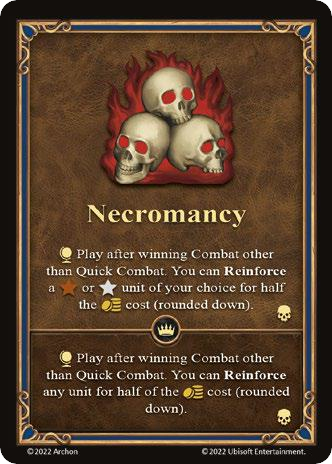
\includegraphics[width=0.25\linewidth]{\images/necromancy_card.png}
\end{figure}
\begin{center}
\small\textit{Cards such as Necromancy allow you to reinforce outside of using the population token.
This does not require owning any of the prerequisite buildings for reinforcing nor flipping your population token.}
\end{center}

\subsection*{Unit card anatomy}

\includesvg[height=30px]{\svgs/attack.svg}\textbf{Attack} – The amount of damage this unit deals when it attacks.
Attacks are always reduced by the defending unit’s defense.
Attacks may be modified by various effects such as the attack die and statistic cards.\par
\includesvg[height=30px]{\svgs/defense.svg}\textbf{Defense} - The amount by which the unit reduces the attack damage it receives.
Does not apply to damage received from spells or other non-attack effects.
Defense may be modified by various effects such as statistic cards.\par
\includesvg[height=30px]{\svgs/HP.svg}\textbf{\hypertarget{HP}{HP}} - The maximum amount of damage a unit can sustain before it is defeated.
”Few” units are discarded from combat and its owner’s unit deck when defeated.
”Pack” units are turned back to ”Few” units, with any excess damage placed on its ”Few” side.
After combat, all damage is healed from all units.
Units retain their ”Few” or ”Pack” status after combat.\par
\includesvg[height=30px]{\svgs/initiative.svg}{\hypertarget{Initiative}{\textbf{Initiative}}} - Determines when the unit activates during combat.
Units with a higher initiative activate first.
In case of a tie, the \hyperlink{Combatterminology}{attacking} side’s unit should always activate first.
If there are multiple ties on one side, the player who controls those units selects which unit to activate next.
If there are multiple ties on both sides (for instance two attackers and two defenders with the same initiative), alternate between the attackers and defenders starting with the attacker.\par
\begin{wrapfigure}{R}{0.5\textwidth}
  \begin{center}
  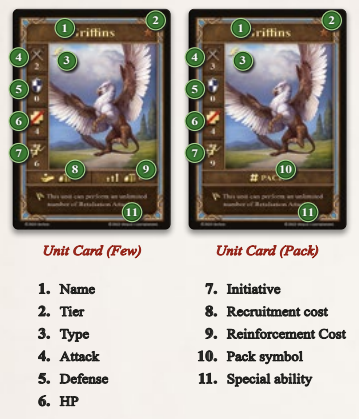
\includegraphics[width=0.48\textwidth]{\images/units.png}
  \end{center}
\end{wrapfigure}
Most units have a \textbf{special ability}:\par

\begin{itemize}[wide]
  \item\textbf{Activation} \includesvg[height=10px]{\svgs/activation.svg} resolves when the unit is activated.
  \item\textbf{Attack} \includesvg[height=10px]{\svgs/unit_attack.svg} resolves when the unit attacks during its activation.
    In case of multiple attacks, resolve the effect for the first attack only.
  \item\textbf{Other} \includesvg[height=10px]{\svgs/unit_other.svg} may be resolved instead of the unit's normal activation.
    Replaces all movement and/or attacking.
  \item\textbf{Passive} \includesvg[height=10px]{\svgs/unit_passive.svg} resolves whenever its condition is met.
  \item\textbf{Retaliate} \includesvg[height=10px]{\svgs/unit_retaliate.svg} resolves when the unit retaliates.
  \item In any cases without one of the above icons, the unit’s ability is used according to its text.
    Units may also have \hyperlink{Playerdecks}{these} symbols.
\end{itemize}

\clearpage
\subsection*{\hypertarget{Unittype}{Unit types}}
There are three types of units:
\begin{itemize}
  \item \textbf{Ground} \includesvg[height=10px]{\svgs/unit_ground.svg} units move up to 3 spaces and attack adjacent enemies.
  \item \textbf{Flying} \includesvg[height=10px]{\svgs/unit_flying.svg} units move up to 3 spaces, ignoring obstacles, and attack adjacent enemies.
  \item \textbf{Ranged} \includesvg[height=10px]{\svgs/unit_ranged.svg} units may attack any unit anywhere and then move 1 space OR move up to 1 space without attacking.
\end{itemize}
If a \includesvg[height=10px]{\svgs/unit_ranged.svg} unit is next to an enemy unit, its attack target must be that adjacent enemy.
When attacking an adjacent enemy in this way the ranged unit suffers a combat penalty: throw two combat dice and \textbf{apply the smaller result}.\par
This penalty is also applied if the \includesvg[height=10px]{\svgs/unit_ranged.svg} unit attacks from its own backline into the enemy's backline.
Walls and gates may also \hyperlink{Walls}{reduce} a ranged unit's attack.

\subsection*{Neutral units}
Neutral units guard the various locations on the game map.
Starting and winning combat against them is necessary to visit most locations.
Neutral units are spread into four different tiers, each with their own deck.
In addition to (\includesvg[height=10px]{\svgs/bronze.svg}, \includesvg[height=10px]{\svgs/silver.svg} and \includesvg[height=10px]{\svgs/golden.svg}, there are also azure \includesvg[height=10px]{\svgs/azure.svg} neutral units which are the strongest in the game.\par
Each of these decks should be kept separate from each other and shuffled during set up.
If a neutral unit deck ever runs out of cards, reshuffle the discard into a new deck.
When a combat against neutral units starts, \hyperlink{Difficulty}{the appropriate number} of units from each tier should be drawn to take part in that combat.\par
It is possible for players to gain neutral units to their unit deck through various effects, such as scenario-specific rules or the diplomacy ability card.
Neutral units cannot be reinforced, as they are single sided.
Whenever a neutral unit is defeated from your unit deck, place it into the neutral discard pile as normal.
\begin{figure}[h]
  \centering
  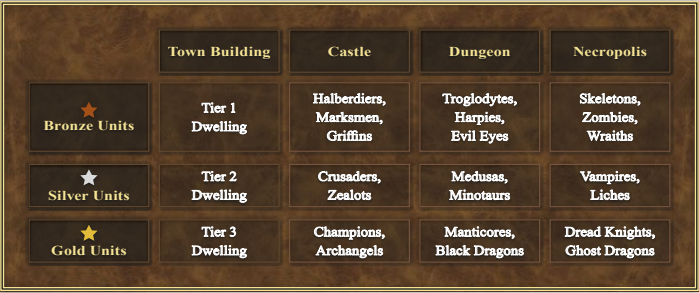
\includegraphics[scale=1]{\images/unit_list.png}
\end{figure}
\begin{center}
  \textit{A graph of all faction units in the core game.}
\end{center}
